%%----------------------------------------------------------------------------
%% Onderzoekstechnieken: Aan de slag (intro)
%%----------------------------------------------------------------------------

\documentclass[aspectratio=169]{beamer}

%==============================================================================
% Aanloop
%==============================================================================

%---------- Vormgeving --------------------------------------------------------

\usetheme{hogent}

\usecolortheme{hgwhite} % witte achtergrond, zwarte tekst

\usepackage{graphicx,multicol}
\usepackage{comment,enumerate,hyperref}
\usepackage{amsmath,amsfonts,amssymb}
\usepackage[english]{babel}
\usepackage{multirow}
\usepackage{eurosym}
\usepackage{listings}
\usepackage{textcomp}
\usepackage{framed}
\usepackage{wrapfig}
\usepackage{booktabs}

%---------- Configuratie ------------------------------------------------------

\usetikzlibrary{arrows,shapes,backgrounds,positioning,shadows}

%---------- Commando-definities -----------------------------------------------

\newcommand{\tabitem}{~~\llap{\textbullet}~~}
\newcommand{\alertbox}[1]{%
  \begin{center}
    \colorbox{hgblue}{\textcolor{white}{\textbf{#1}}}
  \end{center}
}

%---------- Info over de presentatie ------------------------------------------

\title{Chapter 1. Getting Started}
\subtitle{Research Techniques}
\author{Jens Buysse \and Pieter-Jan Maenhaut \and Bert {Van Vreckem}}
\date{AY 2020-2021}

%==============================================================================
% Inhoud presentatie
%==============================================================================

\begin{document}

\begin{frame}
  \maketitle
\end{frame}

\begin{frame}
  \frametitle{What's on the menu?}
  
  \tableofcontents
\end{frame}

\section{Research Techniques}

\begin{frame}
  \frametitle{Research Techniques}
  
  \centering
  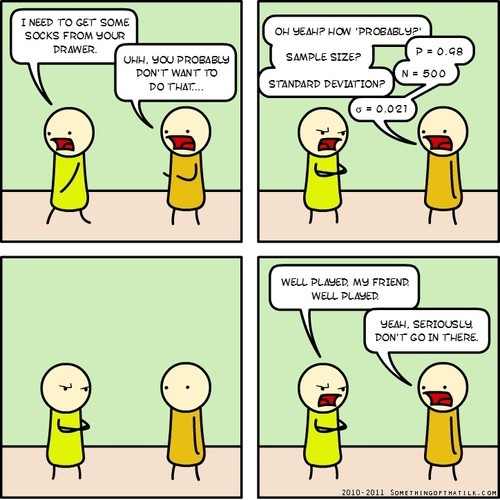
\includegraphics[height=.8\textheight]{intro-01.jpg}
\end{frame}

\begin{frame}
  \frametitle{Purpose}
  
  \begin{itemize}
    \item Introduction to data science / statistics
    \item Preparation for bachelor thesis
  \end{itemize}
\end{frame}

\begin{frame}
  \frametitle{Objectives}
  
  \begin{itemize}
    \item Is able to name and explain concepts, formulas, theorems and their elaboration from \textbf{descriptive and inductive} statistics
    \item Is able to correctly \textbf{apply} formulas and theorems from descriptive and inductive statistics to research questions
    \item Is able to \textbf{analyse} data using statistical software
    \item Is able to \textbf{write} a structured scientific document including references using \LaTeX{}    
    \item Is able to compare the \textbf{scientific method} with non-scientific methods and is able to name advantages and disadvantages
  \end{itemize}
\end{frame}

\begin{frame}
  \frametitle{How Not to Do It}
  
  \centering
  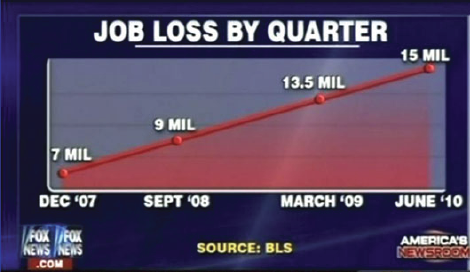
\includegraphics[height=.8\textheight]{intro-02.png}
\end{frame}

\begin{frame}
  \frametitle{How Not to Do It}
  
  \centering
  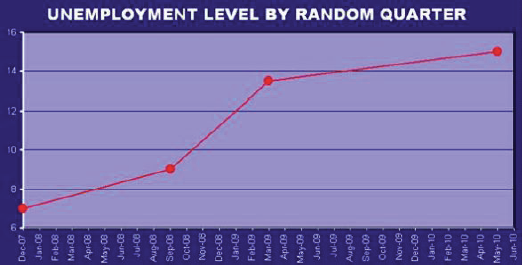
\includegraphics[height=.8\textheight]{intro-03.png}
\end{frame}

\begin{frame}
  \frametitle{How Not to Do It}
  
  \centering
  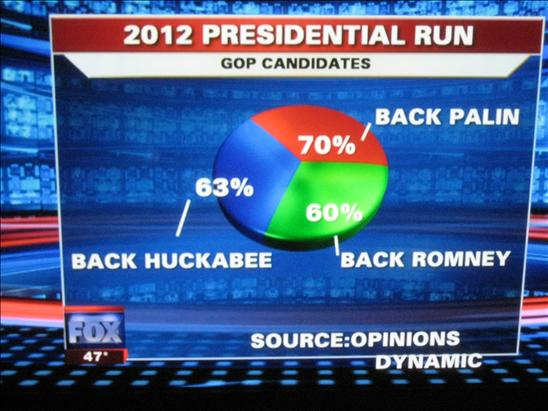
\includegraphics[height=.8\textheight]{intro-04.png}
\end{frame}

\begin{frame}
  \frametitle{How Not to Do It}
  
  \centering
  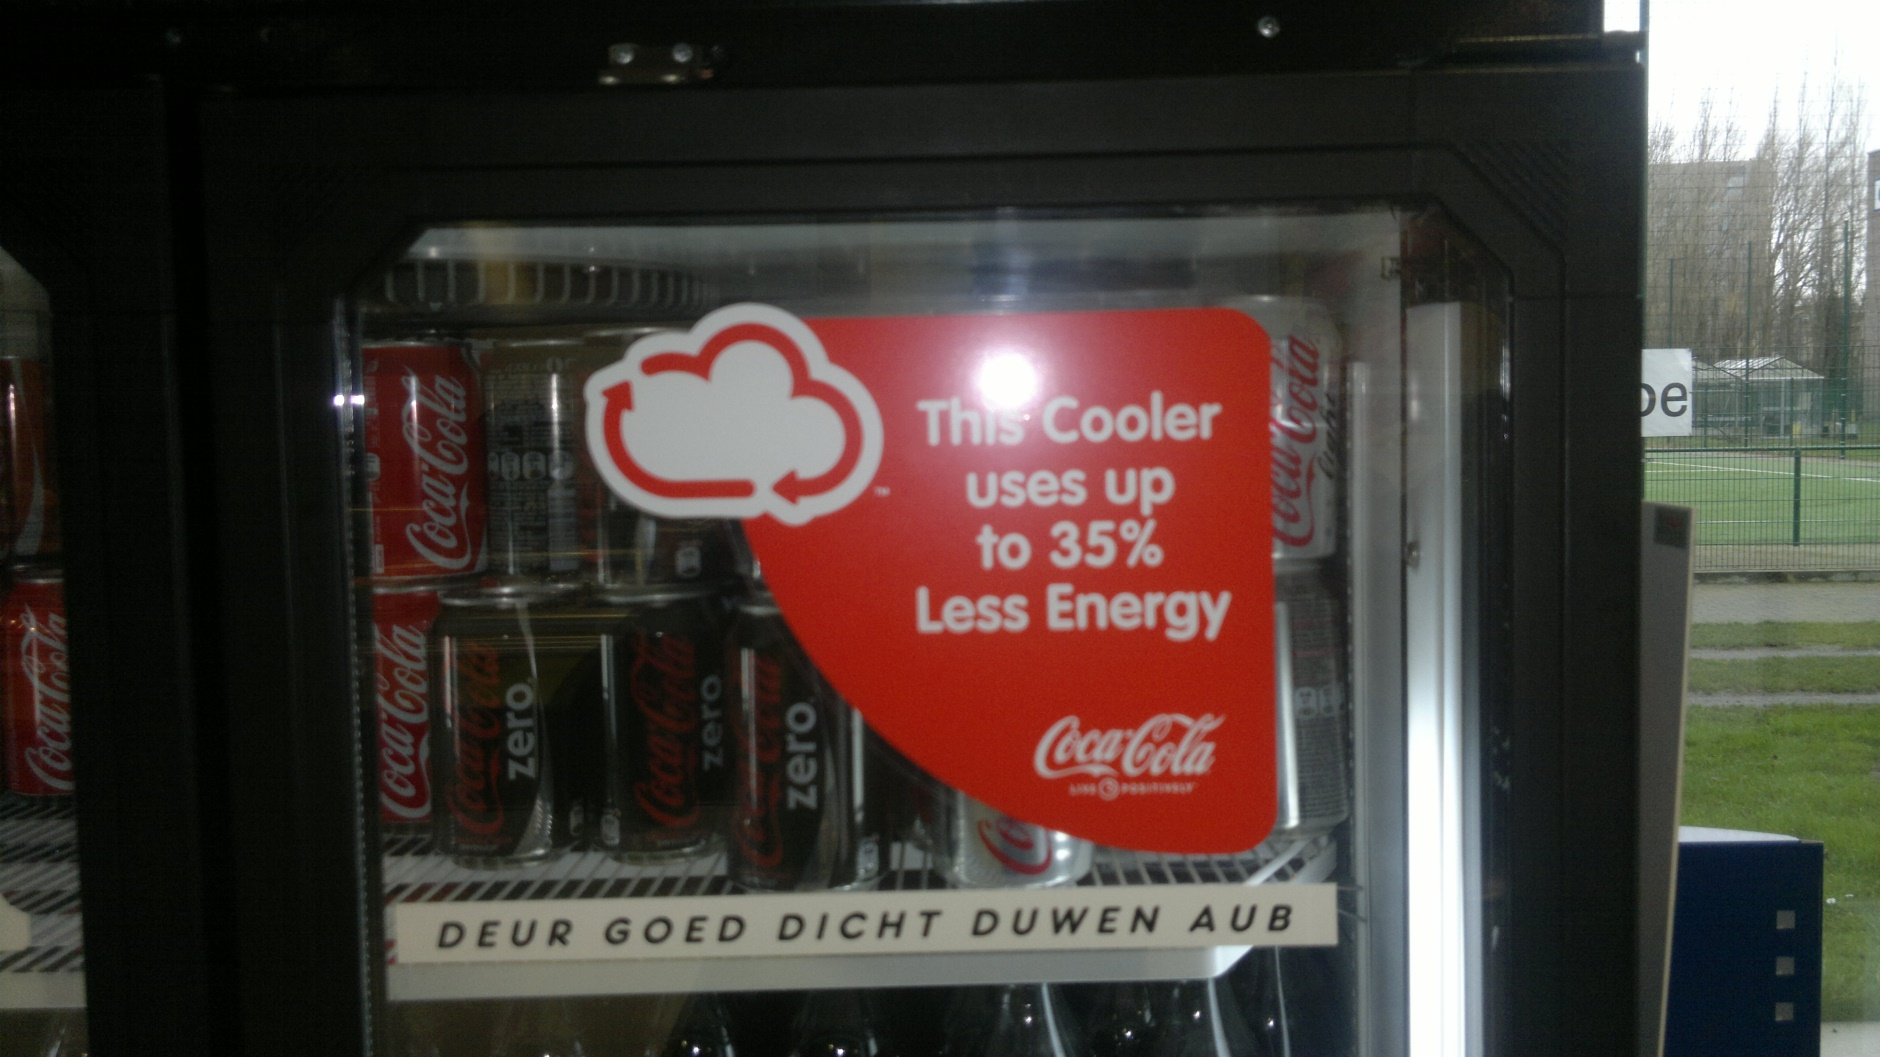
\includegraphics[height=.8\textheight]{intro-05.jpg}
\end{frame}

\begin{frame}
  \frametitle{How Not to Do It}
  
  \centering
  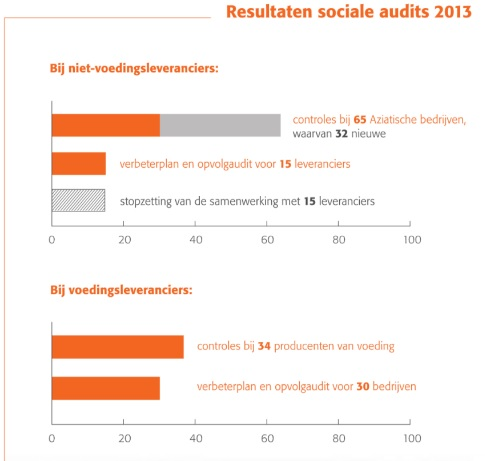
\includegraphics[height=.8\textheight]{intro-10.jpg}
\end{frame}

\begin{frame}
  \frametitle{How Not to Do It}
  
  \begin{figure}
    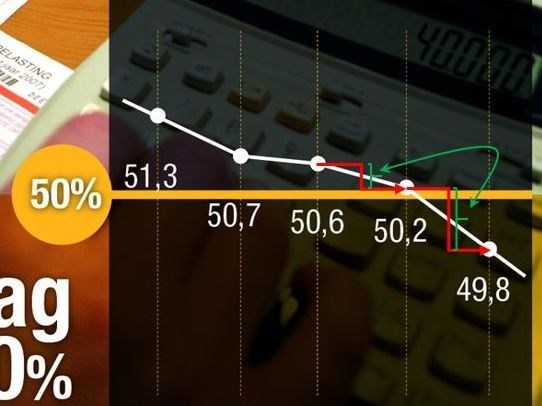
\includegraphics[height=.5\textheight]{intro-nva.jpg}
    \caption{Government demand has fallen last year, but not as spectacular as a chart of the N-VA suggests.
        Economics professor Tom Verbeke noticed this and pointed the finger at N-VA.
        ``If a student would apply such tricks, he would have to defend himself for sure!''}
  \end{figure}
  
\end{frame}

\section{Study Guide}

\begin{frame}{Study Guide}
  All information about this course:
  
  \begin{itemize}
    \item Chamilo
    \item ECTS file: Chamilo or \url{https://www.hogent.be/studiefiches/}
    \item Study Guide: syllabus, Chapter 1. \textit{Getting Started}
  \end{itemize}
\end{frame}

\begin{frame}
  \frametitle{Contents}
  
  \begin{enumerate}
    \item Getting Started
    \item The research process
    \begin{itemize}
      \item The scientific method
      \item Basic concepts, e.g. variables, measurement levels
      \item Sample testing
    \end{itemize}
    \item Univariate analysis
    \begin{itemize}
      \item Center and spread of distribution
      \item Visualization
    \end{itemize}
    \item The central limit theorem
    \begin{itemize}
      \item Probability distribution of a sample
      \item The normal distribution
      \item Confidence intervals
    \end{itemize}
  \end{enumerate}

\end{frame}

\begin{frame}
\frametitle{Contents (cont.)}

  \begin{enumerate}
    \setcounter{enumi}{4}
    \item Review procedures
    \begin{itemize}
      \item Hypothesis tests: basic concepts
      \item Critical area, chance of exceedance
      \item $z$- and $t$-test
    \end{itemize}
    \item Bivariate analysis
    \begin{itemize}
      \item Cross tables and $\chi^2$-test, Cramér's $V$
      \item $t$-test for 2 samples, Cohen's $d$
      \item Regression analysis, correlation
      \item Visualization
    \end{itemize}
    \item Time series
    \begin{itemize}
      \item Time series models and prediction
      \item Moving average
      \item Exponential smoothing, Holt-Winters
    \end{itemize}
  \end{enumerate}
\end{frame}

\begin{frame}
  \frametitle{Study Material}

  \begin{itemize}
    \item Syllabus (PDF on Chamilo, Github)
    \item Slides (PDF)
    \item Github repository containing
    \begin{itemize}
      \item \LaTeX{} source code syllabus, slides
      \item R code examples, tutorials
    \end{itemize}
  \end{itemize}    

\end{frame}

\begin{frame}
  \frametitle{Software}
  
  Instructions: refer to syllabus, Chapter 1.
  
  \begin{itemize}
    \item Git:
    \begin{itemize}
      \item Git client (CLI, GitKraken)
      \item Github Account 
    \end{itemize}
    \item {\LaTeX}:
    \begin{itemize}
      \item MikTeX/MacTeX/Texlive
      \item TexStudio
      \item JabRef (bibliographic database)
    \end{itemize}
    \item Statistics: R, RStudio Desktop
  \end{itemize}
  
  \centering
  All required software is free/open source
\end{frame}

\begin{frame}
  \frametitle{Teaching Methods}
  
  \begin{itemize}
    \item Classroom instructions and lecture (1 hour/week): theory
    \item Exercises and group work (2 hours/week):
    \begin{itemize}
      \item Deepening knowledge
      \item Making exercises
      \item Learn to work with the software
    \end{itemize}
    \item Group work, guided self-study
    \begin{itemize}
      \item Go through a research process
      \item Report on results
    \end{itemize}
    \item Self study
    \begin{itemize}
      \item Study \& exercise!
    \end{itemize}
  \end{itemize}
\end{frame}

\begin{frame}
  \frametitle{Study Tips}
  
  \begin{columns}
    \begin{column}{.8\textwidth}
        The course Research Techniques is often experienced as being difficult
      
      \begin{itemize}
        \item Do not skip the lectures
        \item Take notes actively!
        \item Also spend some time on this subject outside of contact hours
        \item Use good learning techniques
        \item Ask questions!
      \end{itemize}
      
      Some tips are provided in the syllabus
      
    \end{column}
  
    \begin{column}{.2\textwidth}
      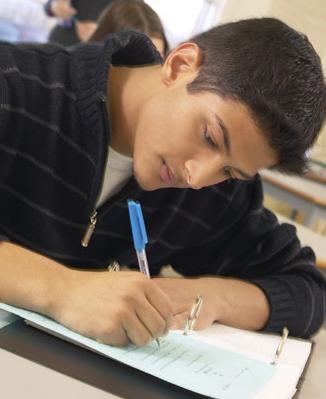
\includegraphics[height=2.5cm]{intro-06.jpg}
    \end{column}
  \end{columns}
  
\end{frame}

\begin{frame}
  \frametitle{Schedule}
  \framesubtitle{Subject to changes due to holidays, etc.}
  
  \centering
  \begin{tabular}{rl}
  	\toprule
  	\textbf{Week} & \textbf{Subject}                \\
  	\midrule
  	            1 & Hst 1 -- Getting Started        \\
  	              & Hst 2 -- Research Process       \\
  	            2 & Hst 2 -- Research Process       \\
  	            3 & Hst 3 -- Univariate analysis    \\
  	            4 & Hst 4 -- Central Limit Theorem  \\
  	            5 & Hst 5 -- Test Procedures        \\
  	            6 & Hst 5 -- Test Procedures        \\
  \end{tabular}
  
\end{frame}

\begin{frame}
  \frametitle{Schedule}
\framesubtitle{Subject to changes due to holidays, etc.}
  
  \centering
  \begin{tabular}{rl}
  	\toprule
  	\textbf{Week} & \textbf{Subject}                                    \\
  	\midrule
  	            7 & Hst 6 -- Bivariate Analysis                         \\
  	              & \hspace{1.25cm} Cross Tables, $\chi^2$ (test)       \\
  	            8 & Hst 6 -- Bivariate Analysis                         \\
  	              & \hspace{1.25cm} $t$-test for 2 samples, effect size \\
  	              & \textbf{Easter holidays}                            \\
  	            9 & Hst 6 -- Bivariate Analysis                         \\
  	              & \hspace{1.25cm} Regression Analysis, Correlation    \\
  	           10 & Hst 7 -- Time Series                                \\
  	           11 & Preparation for bachelor thesis                     \\
  	           12 & Review                                              \\
  \end{tabular}
  
\end{frame}

\begin{frame}
  \frametitle{Evaluation}

  \begin{columns}
    \begin{column}{.8\textwidth}
      \begin{itemize}
        \item First exam chance
        \begin{itemize}
          \item Non-periodic evaluation (NPE, group work): 30\%
          \item Periodic evaluation (exam): 70\%
          \begin{itemize}
            \item 1h closed book (theory)
            \item 1h open book with preparation on own laptop (exercises)
          \end{itemize}
        \end{itemize}
        \item Re-sit Exam
        \begin{itemize}
          \item Non-periodic evaluation: 30\%
          
          \textbf{No second exam opportunity - assesment from first chance will remain valid}
          \item Periodic evaluation: 70\% (same as first exam chance)
        \end{itemize}
      \end{itemize}
    \end{column}
    \begin{column}{.2\textwidth}
      
\includegraphics[height=3cm]{intro-07}
    \end{column}
  \end{columns}

\end{frame}

\begin{frame}
  \frametitle{NPE: Case Study Research Process}
  
  \alertbox{What are determining factors for mathematical proficiency?}
  
  \begin{enumerate}
    \item Literature review
    \item Define research question
    \item Collect resarch results (survey)
    \item Analyze results statistically
    \item Reporting
  \end{enumerate}
  
  Full description on Chamilo, Assignments
\end{frame}

\end{document}